David Rohrbaugh

2014-12-12

The Samantha Module(s), Servos, and the HiTechnic IRSeeker

\begin{tabular}{|p{5cm}|p{5cm}|}
 \hline
 I did a little bit of everything this week as well. I connected each team's robot to the network at least once. I attached a servo controller and connected our goal-grabbing mechansim to it. I also started work on using the HiTechnic IRSeeker.
 &
 All three teams' robots have been connected to the network and controlled from the driver station. Our goal-grabbing mechanism is working, but it will be replaced with something more robust and the continuous rotation servo driving it will be replaced by a normal servo.
 \\
 \hline
\end{tabular}

\medskip

The only things that our team has left to do are making the scoring mechanism and 3D-printing the ramp that directs balls into the scoring mechanism, in addition to lots of testing.

\medskip

Here is a diagram of our current goal-grabbing mechanism:

\begin{center}
 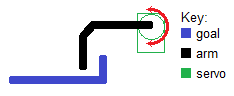
\includegraphics{./Entries/Images/goalGrabber.png}
\end{center}